\chapter{Atomuhr\label{chapter:atomuhr}}
\lhead{Atomuhr}
\begin{refsection}
\chapterauthor{Stefan Steiner und Pascal Stump}

\section{Einleitung}
% Aus Aufgabenstellung A. Müller
%Ein Rubidium-Frequenznormal verwendet eine Eigenschaft von
%Rubidium-Atomen, um ein hochpräzises Frequenznormal ($10^{-11}$)
%bereitzustellen. Solche Frequenznormale werden zum Beispiel in 3G
%Basisstationen oder in Satelliten verwendet.
%
%Es wird erwartet, dass Sie anhand eines vereinfachten Modells
%erklären, wie ein solches Frequenznormal funktioniert. Welche
%äusseren Umstände könnten die Frequenz beeinflussen? Es steht
%ausserdem ein Exemplar eines LPRO-101 für Experimente und Demonstrationen
%zur Verfügung.

Ohne die quantenmechanischen Erkenntnisse, welche besonders zu Beginn des letzten Jahrhunderts gemacht wurden, g"abe es keine Atomuhren. 
Sie stellen eine pr"azise Zeitmessung sicher und ebnen den Weg f"ur immer genauere Messungen in der praktischen Physik. 

Zudem pr"agen diese Ger"ate unseren Alltag, ohne das dies stark bemerkt wird. 
Ortung durch ein Globales Satelliten Navigationssystem (GNSS) wie GPS oder Galileo sind stark von pr"aziser Zeitmessung abh"angig. 
Jeder Satellit diesen Systems beinhaltet eine Atomuhr.
Dies gilt auch f"u das Mobilfunknetz. Die einzelnen Antennen m"ussen untereinander sehr genau synchronisiert sein. Auch da helfen diese genauen Taktgeber.

Dieses Kapitel soll einen kurzen "Uberblick geben, was der Quantenmechanische Hintergrund eines solchen Ger"ates ist. Ausserdem soll die Technische Realisation solch eines Gerätes erläutert werden.
\section{Anwendungen}
% Wie Vortrag -> Bild aus Folie übernehmen...

\section{Quantenmechnanische Betrachtung}

In diesem Kapitel soll erl"autert werden, wie mithilfe der Theorie der Quantenmechanik eine Atomuhr technisch realisiert werden kann. Dabei wird zuerst eine kurze Repetition zum Wasserstoff gegeben, die Feinstruktur erläutert was dann zum Schluss zur Theorie der Hyperfeinstruktur f"uhrt.

\subsection{Repetition Wasserstoffatom}
In Kapitel \ref{chapter:wasserstoff} konnte mithilfe der zeitunabhängigen Schr"odingergleichung hergeleitet werden, dass beim Wasserstoffatom die Entartung gilt.
Dies gilt nicht nur f"ur das Wasserstoffatom, sondern Allgemein.
Das bedeutet, Elektronen können sich nur in einem wohldefinierten Abstand um den Atomkern befinden. 
Diese Erkenntnisse stellte Niels Bohr 1913 mit dem nach ihm benannten Bohrschen Atommodell vor \cite{wiki:bohr}. 

Springt nun ein Elektron von einem tieferen in einen h"oheren Entartungsgrad, so wird ein Photon absorbiert.
Das passiert bei einer Energiezufuhr zum Atom. 
Vice versa sendet das Atom ein Photon aus, wenn ein Elektron von einem h"oheren Energiegrad zu einen tieferen einen Quantensprung vollzieht.

Aus dem Energieunterschied und dem plankschen Wirkungsquantum lässt sich die Frequenz des Photons berechnen
\begin{equation}
	h\nu = \varDelta E.
\end{equation}

\vspace{.5cm}

Aus Tabelle \ref{skript:h2wellenlaengen} sind die Wellenl"angen solcher "Uberg"ange ersichtlich. Daraus sind nun die Photonenfrequenzen zu berechnen.

\begin{center}
	"Ubergang $H\alpha: 3 \rightarrow 2: \lambda_1 = 656.3nm$

$\nu_1 = \dfrac{c}{\lambda_1} = 457.3 THz $
\vspace{.5cm}

"Ubergang $8 \rightarrow 2: \lambda_2 = 388.8nm$

$\nu_2 = \dfrac{c}{\lambda_2} = 771.2 THz$
\end{center}	

Diese "Uberg"ange sind im Berich von Terahertz bis Petahertz und eignen sich darum nicht um sie elektronisch zu verarbeiten.

\begin{figure}[h!]
	\centering
	%TODO im militär ist uploaden teuer, kopiere es dann in den richtigen Ordner, wenn ich zu Hause bin.
	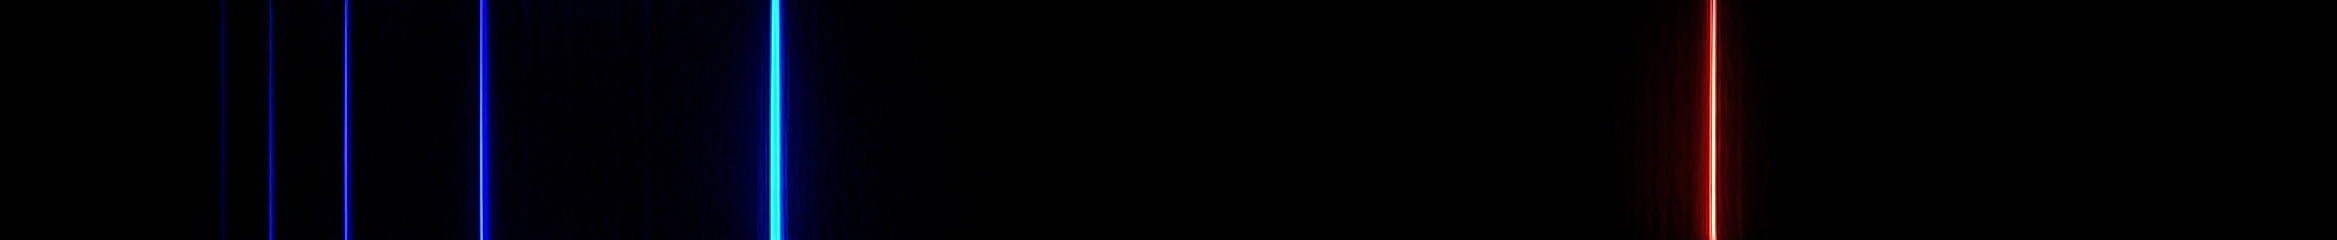
\includegraphics[width = .6\columnwidth]{../vortrag/pictures/wasserstoffSpektrum.jpg}
	\caption{Wasserstoffspektrum} %TODO \cite{link im owncloud ordner}}
\end{figure}


% von einem entartungsgrad in einen anderen springen - photon absorbieren, aussenden.
% Rechnung machen -> H\alpha, 8 \rightarrow 2. Bild wasserstoffspektrum
% 
% Balmer-Serie

%Wasserstoffatom übergang -> im GHz bereich

\subsection{Feinstruktur"ubergang}
Damit jedoch ein solcher "Ubergang elektrisch verarbeitet werden kann, muss es einen Effekt geben, bei welchem das Photon mit einer Frequenz ausgesendet wird, mit der es elektronisch verarbeitet werden kann.
Der Feinstruktur"ubergang ist ein erster Schritt in diese Richtung. 

Als das Wasserstoffspektrum genauer untersuchte wurde, bemerkte man, dass die Spektrallinien nicht atomar sind. Wenn man beispielsweise auf die $H\alpha$ linie stark herein zoomt, entdeckt man, dass diese eine Linie eigentlich zwei sind. 

\begin{figure}[h!]
	\centering
	%TODO im militär ist uploaden teuer, kopiere es dann in den richtigen Ordner, wenn ich zu Hause bin.
	
\includegraphics[width = .6\columnwidth]{../vortrag/pictures/fine_structure_hydrogen.png}
	\caption{$H\alpha$-Linie stark vergrössert} %TODO \cite{link im owncloud ordner}}
\end{figure}

Dieser Effekt ist der Anlass
%Beweis für Elektronenspin
%Bild von übergang

\subsubsection{Notation Termsymbol $^N L _J$}

\subsection{Hyperfeinstrukturübergang}
% Wechselwirkung Elektron <-> Spin
% Rubidium \nu = 6.834 GHz 

\section{Technische Betrachtung}

\subsection{Rechnung}

\section{Ausblick} 

\section{Zusammenfassung}

\printbibliography[heading=subbibliography]
\end{refsection}

